% Created by tikzDevice version 0.10.1 on 2016-08-29 22:50:26
% !TEX encoding = UTF-8 Unicode
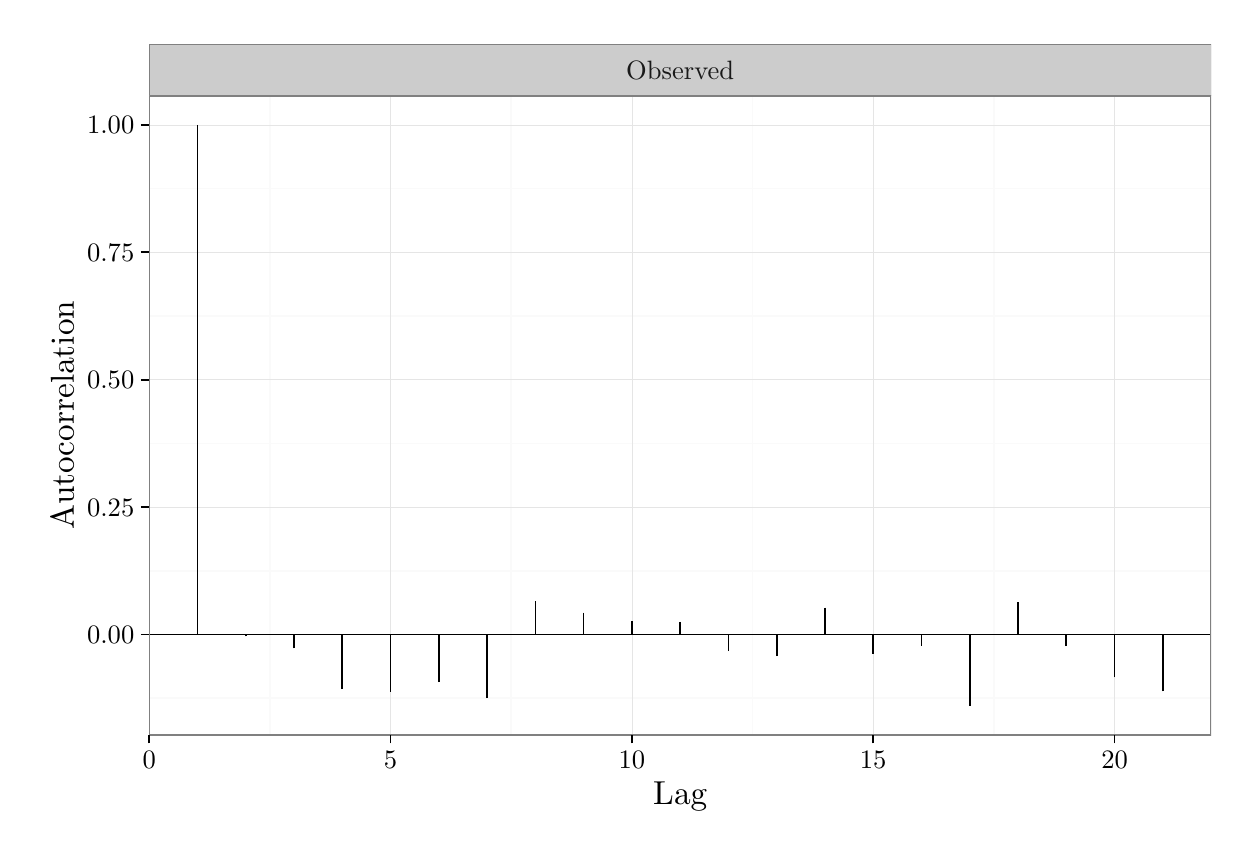
\begin{tikzpicture}[x=1pt,y=1pt]
\definecolor{fillColor}{RGB}{255,255,255}
\path[use as bounding box,fill=fillColor,fill opacity=0.00] (0,0) rectangle (433.62,289.08);
\begin{scope}
\path[clip] (  0.00,  0.00) rectangle (433.62,289.08);
\definecolor{drawColor}{RGB}{255,255,255}
\definecolor{fillColor}{RGB}{255,255,255}

\path[draw=drawColor,line width= 0.6pt,line join=round,line cap=round,fill=fillColor] ( -0.00,  0.00) rectangle (433.62,289.08);
\end{scope}
\begin{scope}
\path[clip] ( 43.93, 33.48) rectangle (427.62,264.47);
\definecolor{fillColor}{RGB}{255,255,255}

\path[fill=fillColor] ( 43.93, 33.48) rectangle (427.62,264.47);
\definecolor{drawColor}{gray}{0.98}

\path[draw=drawColor,line width= 0.6pt,line join=round] ( 43.93, 46.78) --
	(427.62, 46.78);

\path[draw=drawColor,line width= 0.6pt,line join=round] ( 43.93, 92.82) --
	(427.62, 92.82);

\path[draw=drawColor,line width= 0.6pt,line join=round] ( 43.93,138.86) --
	(427.62,138.86);

\path[draw=drawColor,line width= 0.6pt,line join=round] ( 43.93,184.90) --
	(427.62,184.90);

\path[draw=drawColor,line width= 0.6pt,line join=round] ( 43.93,230.95) --
	(427.62,230.95);

\path[draw=drawColor,line width= 0.6pt,line join=round] ( 87.53, 33.48) --
	( 87.53,264.47);

\path[draw=drawColor,line width= 0.6pt,line join=round] (174.73, 33.48) --
	(174.73,264.47);

\path[draw=drawColor,line width= 0.6pt,line join=round] (261.93, 33.48) --
	(261.93,264.47);

\path[draw=drawColor,line width= 0.6pt,line join=round] (349.14, 33.48) --
	(349.14,264.47);
\definecolor{drawColor}{gray}{0.90}

\path[draw=drawColor,line width= 0.2pt,line join=round] ( 43.93, 69.80) --
	(427.62, 69.80);

\path[draw=drawColor,line width= 0.2pt,line join=round] ( 43.93,115.84) --
	(427.62,115.84);

\path[draw=drawColor,line width= 0.2pt,line join=round] ( 43.93,161.88) --
	(427.62,161.88);

\path[draw=drawColor,line width= 0.2pt,line join=round] ( 43.93,207.93) --
	(427.62,207.93);

\path[draw=drawColor,line width= 0.2pt,line join=round] ( 43.93,253.97) --
	(427.62,253.97);

\path[draw=drawColor,line width= 0.2pt,line join=round] ( 43.93, 33.48) --
	( 43.93,264.47);

\path[draw=drawColor,line width= 0.2pt,line join=round] (131.13, 33.48) --
	(131.13,264.47);

\path[draw=drawColor,line width= 0.2pt,line join=round] (218.33, 33.48) --
	(218.33,264.47);

\path[draw=drawColor,line width= 0.2pt,line join=round] (305.54, 33.48) --
	(305.54,264.47);

\path[draw=drawColor,line width= 0.2pt,line join=round] (392.74, 33.48) --
	(392.74,264.47);
\definecolor{drawColor}{RGB}{0,0,0}

\path[draw=drawColor,line width= 0.6pt,line join=round] ( 43.93, 69.80) -- (427.62, 69.80);

\path[draw=drawColor,line width= 0.6pt,line join=round] ( 61.37,253.97) -- ( 61.37, 69.80);

\path[draw=drawColor,line width= 0.6pt,line join=round] ( 78.81, 69.12) -- ( 78.81, 69.80);

\path[draw=drawColor,line width= 0.6pt,line join=round] ( 96.25, 64.82) -- ( 96.25, 69.80);

\path[draw=drawColor,line width= 0.6pt,line join=round] (113.69, 50.03) -- (113.69, 69.80);

\path[draw=drawColor,line width= 0.6pt,line join=round] (131.13, 49.06) -- (131.13, 69.80);

\path[draw=drawColor,line width= 0.6pt,line join=round] (148.57, 52.60) -- (148.57, 69.80);

\path[draw=drawColor,line width= 0.6pt,line join=round] (166.01, 46.83) -- (166.01, 69.80);

\path[draw=drawColor,line width= 0.6pt,line join=round] (183.45, 81.76) -- (183.45, 69.80);

\path[draw=drawColor,line width= 0.6pt,line join=round] (200.89, 77.72) -- (200.89, 69.80);

\path[draw=drawColor,line width= 0.6pt,line join=round] (218.33, 74.58) -- (218.33, 69.80);

\path[draw=drawColor,line width= 0.6pt,line join=round] (235.77, 74.34) -- (235.77, 69.80);

\path[draw=drawColor,line width= 0.6pt,line join=round] (253.21, 63.81) -- (253.21, 69.80);

\path[draw=drawColor,line width= 0.6pt,line join=round] (270.65, 62.00) -- (270.65, 69.80);

\path[draw=drawColor,line width= 0.6pt,line join=round] (288.10, 79.52) -- (288.10, 69.80);

\path[draw=drawColor,line width= 0.6pt,line join=round] (305.54, 62.85) -- (305.54, 69.80);

\path[draw=drawColor,line width= 0.6pt,line join=round] (322.98, 65.73) -- (322.98, 69.80);

\path[draw=drawColor,line width= 0.6pt,line join=round] (340.42, 43.98) -- (340.42, 69.80);

\path[draw=drawColor,line width= 0.6pt,line join=round] (357.86, 81.46) -- (357.86, 69.80);

\path[draw=drawColor,line width= 0.6pt,line join=round] (375.30, 65.57) -- (375.30, 69.80);

\path[draw=drawColor,line width= 0.6pt,line join=round] (392.74, 54.29) -- (392.74, 69.80);

\path[draw=drawColor,line width= 0.6pt,line join=round] (410.18, 49.25) -- (410.18, 69.80);
\definecolor{drawColor}{gray}{0.50}

\path[draw=drawColor,line width= 0.6pt,line join=round,line cap=round] ( 43.93, 33.48) rectangle (427.62,264.47);
\end{scope}
\begin{scope}
\path[clip] ( 43.93,264.47) rectangle (427.62,283.08);
\definecolor{drawColor}{gray}{0.50}
\definecolor{fillColor}{gray}{0.80}

\path[draw=drawColor,line width= 0.2pt,line join=round,line cap=round,fill=fillColor] ( 43.93,264.47) rectangle (427.62,283.08);
\definecolor{drawColor}{gray}{0.10}

\node[text=drawColor,anchor=base,inner sep=0pt, outer sep=0pt, scale=  0.96] at (235.77,270.47) {Observed};
\end{scope}
\begin{scope}
\path[clip] (  0.00,  0.00) rectangle (433.62,289.08);
\definecolor{drawColor}{RGB}{0,0,0}

\node[text=drawColor,anchor=base east,inner sep=0pt, outer sep=0pt, scale=  0.96] at ( 38.53, 66.49) {0.00};

\node[text=drawColor,anchor=base east,inner sep=0pt, outer sep=0pt, scale=  0.96] at ( 38.53,112.53) {0.25};

\node[text=drawColor,anchor=base east,inner sep=0pt, outer sep=0pt, scale=  0.96] at ( 38.53,158.58) {0.50};

\node[text=drawColor,anchor=base east,inner sep=0pt, outer sep=0pt, scale=  0.96] at ( 38.53,204.62) {0.75};

\node[text=drawColor,anchor=base east,inner sep=0pt, outer sep=0pt, scale=  0.96] at ( 38.53,250.66) {1.00};
\end{scope}
\begin{scope}
\path[clip] (  0.00,  0.00) rectangle (433.62,289.08);
\definecolor{drawColor}{RGB}{0,0,0}

\path[draw=drawColor,line width= 0.6pt,line join=round] ( 40.93, 69.80) --
	( 43.93, 69.80);

\path[draw=drawColor,line width= 0.6pt,line join=round] ( 40.93,115.84) --
	( 43.93,115.84);

\path[draw=drawColor,line width= 0.6pt,line join=round] ( 40.93,161.88) --
	( 43.93,161.88);

\path[draw=drawColor,line width= 0.6pt,line join=round] ( 40.93,207.93) --
	( 43.93,207.93);

\path[draw=drawColor,line width= 0.6pt,line join=round] ( 40.93,253.97) --
	( 43.93,253.97);
\end{scope}
\begin{scope}
\path[clip] (  0.00,  0.00) rectangle (433.62,289.08);
\definecolor{drawColor}{RGB}{0,0,0}

\path[draw=drawColor,line width= 0.6pt,line join=round] ( 43.93, 30.48) --
	( 43.93, 33.48);

\path[draw=drawColor,line width= 0.6pt,line join=round] (131.13, 30.48) --
	(131.13, 33.48);

\path[draw=drawColor,line width= 0.6pt,line join=round] (218.33, 30.48) --
	(218.33, 33.48);

\path[draw=drawColor,line width= 0.6pt,line join=round] (305.54, 30.48) --
	(305.54, 33.48);

\path[draw=drawColor,line width= 0.6pt,line join=round] (392.74, 30.48) --
	(392.74, 33.48);
\end{scope}
\begin{scope}
\path[clip] (  0.00,  0.00) rectangle (433.62,289.08);
\definecolor{drawColor}{RGB}{0,0,0}

\node[text=drawColor,anchor=base,inner sep=0pt, outer sep=0pt, scale=  0.96] at ( 43.93, 21.46) {0};

\node[text=drawColor,anchor=base,inner sep=0pt, outer sep=0pt, scale=  0.96] at (131.13, 21.46) {5};

\node[text=drawColor,anchor=base,inner sep=0pt, outer sep=0pt, scale=  0.96] at (218.33, 21.46) {10};

\node[text=drawColor,anchor=base,inner sep=0pt, outer sep=0pt, scale=  0.96] at (305.54, 21.46) {15};

\node[text=drawColor,anchor=base,inner sep=0pt, outer sep=0pt, scale=  0.96] at (392.74, 21.46) {20};
\end{scope}
\begin{scope}
\path[clip] (  0.00,  0.00) rectangle (433.62,289.08);
\definecolor{drawColor}{RGB}{0,0,0}

\node[text=drawColor,anchor=base,inner sep=0pt, outer sep=0pt, scale=  1.20] at (235.77,  8.40) {Lag};
\end{scope}
\begin{scope}
\path[clip] (  0.00,  0.00) rectangle (433.62,289.08);
\definecolor{drawColor}{RGB}{0,0,0}

\node[text=drawColor,rotate= 90.00,anchor=base,inner sep=0pt, outer sep=0pt, scale=  1.20] at ( 16.66,148.97) {Autocorrelation};
\end{scope}
\end{tikzpicture}
